\documentclass[1p]{elsarticle_modified}
%\bibliographystyle{elsarticle-num}

%\usepackage[colorlinks]{hyperref}
%\usepackage{abbrmath_seonhwa} %\Abb, \Ascr, \Acal ,\Abf, \Afrak
\usepackage{amsfonts}
\usepackage{amssymb}
\usepackage{amsmath}
\usepackage{amsthm}
\usepackage{scalefnt}
\usepackage{amsbsy}
\usepackage{kotex}
\usepackage{caption}
\usepackage{subfig}
\usepackage{color}
\usepackage{graphicx}
\usepackage{xcolor} %% white, black, red, green, blue, cyan, magenta, yellow
\usepackage{float}
\usepackage{setspace}
\usepackage{hyperref}

\usepackage{tikz}
\usetikzlibrary{arrows}

\usepackage{multirow}
\usepackage{array} % fixed length table
\usepackage{hhline}

%%%%%%%%%%%%%%%%%%%%%
\makeatletter
\renewcommand*\env@matrix[1][\arraystretch]{%
	\edef\arraystretch{#1}%
	\hskip -\arraycolsep
	\let\@ifnextchar\new@ifnextchar
	\array{*\c@MaxMatrixCols c}}
\makeatother %https://tex.stackexchange.com/questions/14071/how-can-i-increase-the-line-spacing-in-a-matrix
%%%%%%%%%%%%%%%

\usepackage[normalem]{ulem}

\newcommand{\msout}[1]{\ifmmode\text{\sout{\ensuremath{#1}}}\else\sout{#1}\fi}
%SOURCE: \msout is \stkout macro in https://tex.stackexchange.com/questions/20609/strikeout-in-math-mode

\newcommand{\cancel}[1]{
	\ifmmode
	{\color{red}\msout{#1}}
	\else
	{\color{red}\sout{#1}}
	\fi
}

\newcommand{\add}[1]{
	{\color{blue}\uwave{#1}}
}

\newcommand{\replace}[2]{
	\ifmmode
	{\color{red}\msout{#1}}{\color{blue}\uwave{#2}}
	\else
	{\color{red}\sout{#1}}{\color{blue}\uwave{#2}}
	\fi
}

\newcommand{\Sol}{\mathcal{S}} %segment
\newcommand{\D}{D} %diagram
\newcommand{\A}{\mathcal{A}} %arc


%%%%%%%%%%%%%%%%%%%%%%%%%%%%%5 test

\def\sl{\operatorname{\textup{SL}}(2,\Cbb)}
\def\psl{\operatorname{\textup{PSL}}(2,\Cbb)}
\def\quan{\mkern 1mu \triangleright \mkern 1mu}

\theoremstyle{definition}
\newtheorem{thm}{Theorem}[section]
\newtheorem{prop}[thm]{Proposition}
\newtheorem{lem}[thm]{Lemma}
\newtheorem{ques}[thm]{Question}
\newtheorem{cor}[thm]{Corollary}
\newtheorem{defn}[thm]{Definition}
\newtheorem{exam}[thm]{Example}
\newtheorem{rmk}[thm]{Remark}
\newtheorem{alg}[thm]{Algorithm}

\newcommand{\I}{\sqrt{-1}}
\begin{document}

%\begin{frontmatter}
%
%\title{Boundary parabolic representations of knots up to 8 crossings}
%
%%% Group authors per affiliation:
%\author{Yunhi Cho} 
%\address{Department of Mathematics, University of Seoul, Seoul, Korea}
%\ead{yhcho@uos.ac.kr}
%
%
%\author{Seonhwa Kim} %\fnref{s_kim}}
%\address{Center for Geometry and Physics, Institute for Basic Science, Pohang, 37673, Korea}
%\ead{ryeona17@ibs.re.kr}
%
%\author{Hyuk Kim}
%\address{Department of Mathematical Sciences, Seoul National University, Seoul 08826, Korea}
%\ead{hyukkim@snu.ac.kr}
%
%\author{Seokbeom Yoon}
%\address{Department of Mathematical Sciences, Seoul National University, Seoul, 08826,  Korea}
%\ead{sbyoon15@snu.ac.kr}
%
%\begin{abstract}
%We find all boundary parabolic representation of knots up to 8 crossings.
%
%\end{abstract}
%\begin{keyword}
%    \MSC[2010] 57M25 
%\end{keyword}
%
%\end{frontmatter}

%\linenumbers
%\tableofcontents
%
\newcommand\colored[1]{\textcolor{white}{\rule[-0.35ex]{0.8em}{1.4ex}}\kern-0.8em\color{red} #1}%
%\newcommand\colored[1]{\textcolor{white}{ #1}\kern-2.17ex	\textcolor{white}{ #1}\kern-1.81ex	\textcolor{white}{ #1}\kern-2.15ex\color{red}#1	}

{\Large $\underline{12n_{0786}~(K12n_{0786})}$}

\setlength{\tabcolsep}{10pt}
\renewcommand{\arraystretch}{1.6}
\vspace{1cm}\begin{tabular}{m{100pt}>{\centering\arraybackslash}m{274pt}}
\multirow{5}{120pt}{
	\centering
	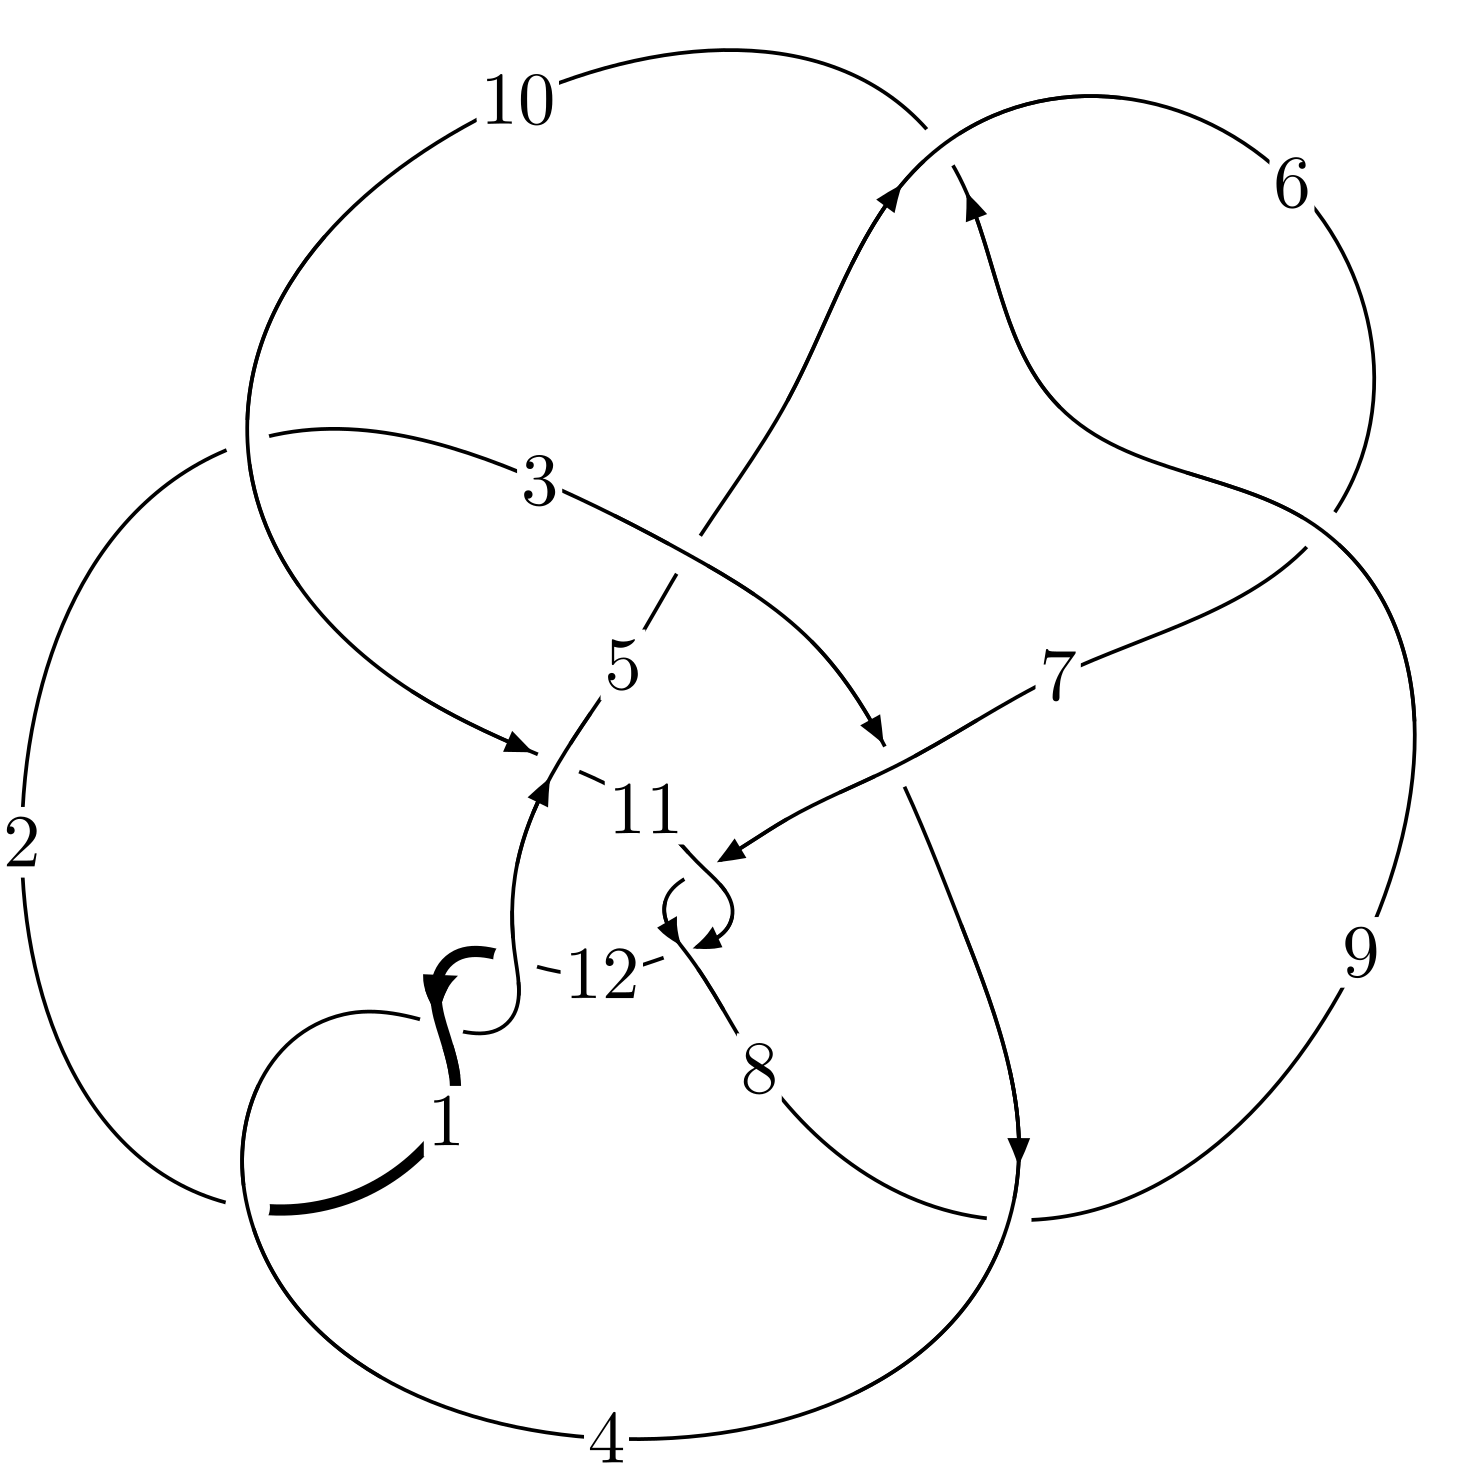
\includegraphics[width=112pt]{../../../GIT/diagram.site/Diagrams/png/2875_12n_0786.png}\\
\ \ \ A knot diagram\footnotemark}&
\allowdisplaybreaks
\textbf{Linearized knot diagam} \\
\cline{2-2}
 &
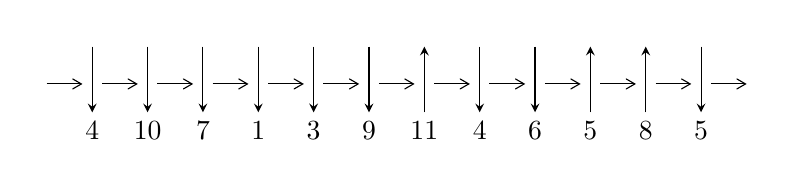
\begin{tikzpicture}[x=20pt, y=17pt]
	% nodes
	\node (C0) at (0, 0) {};
	\node (C1) at (1, 0) {};
	\node (C1U) at (1, +1) {};
	\node (C1D) at (1, -1) {4};

	\node (C2) at (2, 0) {};
	\node (C2U) at (2, +1) {};
	\node (C2D) at (2, -1) {10};

	\node (C3) at (3, 0) {};
	\node (C3U) at (3, +1) {};
	\node (C3D) at (3, -1) {7};

	\node (C4) at (4, 0) {};
	\node (C4U) at (4, +1) {};
	\node (C4D) at (4, -1) {1};

	\node (C5) at (5, 0) {};
	\node (C5U) at (5, +1) {};
	\node (C5D) at (5, -1) {3};

	\node (C6) at (6, 0) {};
	\node (C6U) at (6, +1) {};
	\node (C6D) at (6, -1) {9};

	\node (C7) at (7, 0) {};
	\node (C7U) at (7, +1) {};
	\node (C7D) at (7, -1) {11};

	\node (C8) at (8, 0) {};
	\node (C8U) at (8, +1) {};
	\node (C8D) at (8, -1) {4};

	\node (C9) at (9, 0) {};
	\node (C9U) at (9, +1) {};
	\node (C9D) at (9, -1) {6};

	\node (C10) at (10, 0) {};
	\node (C10U) at (10, +1) {};
	\node (C10D) at (10, -1) {5};

	\node (C11) at (11, 0) {};
	\node (C11U) at (11, +1) {};
	\node (C11D) at (11, -1) {8};

	\node (C12) at (12, 0) {};
	\node (C12U) at (12, +1) {};
	\node (C12D) at (12, -1) {5};
	\node (C13) at (13, 0) {};

	% arrows
	\draw[->,>={angle 60}]
	(C0) edge (C1) (C1) edge (C2) (C2) edge (C3) (C3) edge (C4) (C4) edge (C5) (C5) edge (C6) (C6) edge (C7) (C7) edge (C8) (C8) edge (C9) (C9) edge (C10) (C10) edge (C11) (C11) edge (C12) (C12) edge (C13) ;	\draw[->,>=stealth]
	(C1U) edge (C1D) (C2U) edge (C2D) (C3U) edge (C3D) (C4U) edge (C4D) (C5U) edge (C5D) (C6U) edge (C6D) (C7D) edge (C7U) (C8U) edge (C8D) (C9U) edge (C9D) (C10D) edge (C10U) (C11D) edge (C11U) (C12U) edge (C12D) ;
	\end{tikzpicture} \\
\hhline{~~} \\& 
\textbf{Solving Sequence} \\ \cline{2-2} 
 &
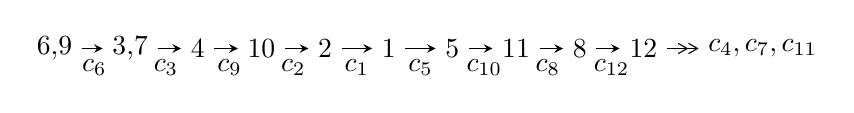
\begin{tikzpicture}[x=23pt, y=7pt]
	% node
	\node (A0) at (-1/8, 0) {6,9};
	\node (A1) at (17/16, 0) {3,7};
	\node (A2) at (17/8, 0) {4};
	\node (A3) at (25/8, 0) {10};
	\node (A4) at (33/8, 0) {2};
	\node (A5) at (41/8, 0) {1};
	\node (A6) at (49/8, 0) {5};
	\node (A7) at (57/8, 0) {11};
	\node (A8) at (65/8, 0) {8};
	\node (A9) at (73/8, 0) {12};
	\node (C1) at (1/2, -1) {$c_{6}$};
	\node (C2) at (13/8, -1) {$c_{3}$};
	\node (C3) at (21/8, -1) {$c_{9}$};
	\node (C4) at (29/8, -1) {$c_{2}$};
	\node (C5) at (37/8, -1) {$c_{1}$};
	\node (C6) at (45/8, -1) {$c_{5}$};
	\node (C7) at (53/8, -1) {$c_{10}$};
	\node (C8) at (61/8, -1) {$c_{8}$};
	\node (C9) at (69/8, -1) {$c_{12}$};
	\node (A10) at (11, 0) {$c_{4},c_{7},c_{11}$};

	% edge
	\draw[->,>=stealth]	
	(A0) edge (A1) (A1) edge (A2) (A2) edge (A3) (A3) edge (A4) (A4) edge (A5) (A5) edge (A6) (A6) edge (A7) (A7) edge (A8) (A8) edge (A9) ;
	\draw[->>,>={angle 60}]	
	(A9) edge (A10);
\end{tikzpicture} \\ 

\end{tabular} \\

\footnotetext{
The image of knot diagram is generated by the software ``\textbf{Draw programme}" developed by Andrew Bartholomew(\url{http://www.layer8.co.uk/maths/draw/index.htm\#Running-draw}), where we modified some parts for our purpose(\url{https://github.com/CATsTAILs/LinksPainter}).
}\phantom \\ \newline 
\centering \textbf{Ideals for irreducible components\footnotemark of $X_{\text{par}}$} 
 
\begin{align*}
I^u_{1}&=\langle 
1.92258\times10^{217} u^{92}-1.17339\times10^{215} u^{91}+\cdots+5.50269\times10^{214} b+4.31038\times10^{217},\\
\phantom{I^u_{1}}&\phantom{= \langle  }-1.20339\times10^{218} u^{92}-2.33162\times10^{218} u^{91}+\cdots+5.50269\times10^{214} a+5.33906\times10^{217},\\
\phantom{I^u_{1}}&\phantom{= \langle  }u^{93}+2 u^{92}+\cdots+3 u-1\rangle \\
I^u_{2}&=\langle 
-10608396395 u^{23}+16008040214 u^{22}+\cdots+27133411469 b+6807317624,\\
\phantom{I^u_{2}}&\phantom{= \langle  }-39241331316 u^{23}-4066209209 u^{22}+\cdots+27133411469 a-90858330224,\\
\phantom{I^u_{2}}&\phantom{= \langle  }u^{24}- u^{23}+\cdots-6 u+1\rangle \\
\\
\end{align*}
\raggedright * 2 irreducible components of $\dim_{\mathbb{C}}=0$, with total 117 representations.\\
\footnotetext{All coefficients of polynomials are rational numbers. But the coefficients are sometimes approximated in decimal forms when there is not enough margin.}
\newpage
\renewcommand{\arraystretch}{1}
\centering \section*{I. $I^u_{1}= \langle 1.92\times10^{217} u^{92}-1.17\times10^{215} u^{91}+\cdots+5.50\times10^{214} b+4.31\times10^{217},\;-1.20\times10^{218} u^{92}-2.33\times10^{218} u^{91}+\cdots+5.50\times10^{214} a+5.34\times10^{217},\;u^{93}+2 u^{92}+\cdots+3 u-1 \rangle$}
\flushleft \textbf{(i) Arc colorings}\\
\begin{tabular}{m{7pt} m{180pt} m{7pt} m{180pt} }
\flushright $a_{6}=$&$\begin{pmatrix}1\\0\end{pmatrix}$ \\
\flushright $a_{9}=$&$\begin{pmatrix}0\\u\end{pmatrix}$ \\
\flushright $a_{3}=$&$\begin{pmatrix}2186.92 u^{92}+4237.23 u^{91}+\cdots+494.015 u-970.264\\-349.390 u^{92}+2.13239 u^{91}+\cdots+3262.94 u-783.323\end{pmatrix}$ \\
\flushright $a_{7}=$&$\begin{pmatrix}1\\u^2\end{pmatrix}$ \\
\flushright $a_{4}=$&$\begin{pmatrix}970.001 u^{92}+1817.60 u^{91}+\cdots-172.176 u-323.551\\555.549 u^{92}+1430.31 u^{91}+\cdots+2003.40 u-769.116\end{pmatrix}$ \\
\flushright $a_{10}=$&$\begin{pmatrix}- u\\u\end{pmatrix}$ \\
\flushright $a_{2}=$&$\begin{pmatrix}594.533 u^{92}+1273.52 u^{91}+\cdots+638.636 u-405.961\\1243.00 u^{92}+2965.84 u^{91}+\cdots+3118.32 u-1347.63\end{pmatrix}$ \\
\flushright $a_{1}=$&$\begin{pmatrix}-268.181 u^{92}-747.988 u^{91}+\cdots-1064.88 u+427.216\\727.736 u^{92}+835.981 u^{91}+\cdots-2598.74 u+446.237\end{pmatrix}$ \\
\flushright $a_{5}=$&$\begin{pmatrix}1040.25 u^{92}+2073.37 u^{91}+\cdots+381.277 u-545.222\\-952.405 u^{92}-1172.41 u^{91}+\cdots+3191.51 u-513.832\end{pmatrix}$ \\
\flushright $a_{11}=$&$\begin{pmatrix}1807.51 u^{92}+4783.68 u^{91}+\cdots+6936.30 u-2674.48\\-1482.28 u^{92}-2741.56 u^{91}+\cdots+115.240 u+560.669\end{pmatrix}$ \\
\flushright $a_{8}=$&$\begin{pmatrix}-1.82342 u^{92}-1725.47 u^{91}+\cdots-8721.80 u+2453.86\\-157.679 u^{92}+622.832 u^{91}+\cdots+4658.44 u-1262.27\end{pmatrix}$ \\
\flushright $a_{12}=$&$\begin{pmatrix}-1467.45 u^{92}-3084.65 u^{91}+\cdots-1415.77 u+1033.53\\2134.10 u^{92}+3027.40 u^{91}+\cdots-4950.71 u+536.369\end{pmatrix}$\\&\end{tabular}
\flushleft \textbf{(ii) Obstruction class $= -1$}\\~\\
\flushleft \textbf{(iii) Cusp Shapes $= -3053.46 u^{92}-12740.4 u^{91}+\cdots-33773.0 u+10600.2$}\\~\\
\newpage\renewcommand{\arraystretch}{1}
\flushleft \textbf{(iv) u-Polynomials at the component}\newline \\
\begin{tabular}{m{50pt}|m{274pt}}
Crossings & \hspace{64pt}u-Polynomials at each crossing \\
\hline $$\begin{aligned}c_{1},c_{4},c_{12}\end{aligned}$$&$\begin{aligned}
&u^{93}+7 u^{92}+\cdots+36 u+31
\end{aligned}$\\
\hline $$\begin{aligned}c_{2}\end{aligned}$$&$\begin{aligned}
&u^{93}-6 u^{92}+\cdots+2531 u+103
\end{aligned}$\\
\hline $$\begin{aligned}c_{3}\end{aligned}$$&$\begin{aligned}
&u^{93}+4 u^{91}+\cdots-30 u+1
\end{aligned}$\\
\hline $$\begin{aligned}c_{5}\end{aligned}$$&$\begin{aligned}
&u^{93}-3 u^{92}+\cdots-22 u+3
\end{aligned}$\\
\hline $$\begin{aligned}c_{6},c_{9}\end{aligned}$$&$\begin{aligned}
&u^{93}-2 u^{92}+\cdots+3 u+1
\end{aligned}$\\
\hline $$\begin{aligned}c_{7},c_{11}\end{aligned}$$&$\begin{aligned}
&u^{93}-6 u^{92}+\cdots-33 u+1
\end{aligned}$\\
\hline $$\begin{aligned}c_{8}\end{aligned}$$&$\begin{aligned}
&u^{93}- u^{92}+\cdots+3067 u+1049
\end{aligned}$\\
\hline $$\begin{aligned}c_{10}\end{aligned}$$&$\begin{aligned}
&u^{93}+5 u^{92}+\cdots+48499913 u+3071059
\end{aligned}$\\
\hline
\end{tabular}\\~\\
\newpage\renewcommand{\arraystretch}{1}
\flushleft \textbf{(v) Riley Polynomials at the component}\newline \\
\begin{tabular}{m{50pt}|m{274pt}}
Crossings & \hspace{64pt}Riley Polynomials at each crossing \\
\hline $$\begin{aligned}c_{1},c_{4},c_{12}\end{aligned}$$&$\begin{aligned}
&y^{93}+33 y^{92}+\cdots-32556 y-961
\end{aligned}$\\
\hline $$\begin{aligned}c_{2}\end{aligned}$$&$\begin{aligned}
&y^{93}-12 y^{92}+\cdots+3176499 y-10609
\end{aligned}$\\
\hline $$\begin{aligned}c_{3}\end{aligned}$$&$\begin{aligned}
&y^{93}+8 y^{92}+\cdots+98 y-1
\end{aligned}$\\
\hline $$\begin{aligned}c_{5}\end{aligned}$$&$\begin{aligned}
&y^{93}+7 y^{92}+\cdots+316 y-9
\end{aligned}$\\
\hline $$\begin{aligned}c_{6},c_{9}\end{aligned}$$&$\begin{aligned}
&y^{93}+60 y^{92}+\cdots-39 y-1
\end{aligned}$\\
\hline $$\begin{aligned}c_{7},c_{11}\end{aligned}$$&$\begin{aligned}
&y^{93}-32 y^{92}+\cdots+605 y-1
\end{aligned}$\\
\hline $$\begin{aligned}c_{8}\end{aligned}$$&$\begin{aligned}
&y^{93}-17 y^{92}+\cdots-40616125 y-1100401
\end{aligned}$\\
\hline $$\begin{aligned}c_{10}\end{aligned}$$&$\begin{aligned}
&y^{93}+39 y^{92}+\cdots-302038266937865 y-9431403381481
\end{aligned}$\\
\hline
\end{tabular}\\~\\
\newpage\flushleft \textbf{(vi) Complex Volumes and Cusp Shapes}
$$\begin{array}{c|c|c}  
\text{Solutions to }I^u_{1}& \I (\text{vol} + \sqrt{-1}CS) & \text{Cusp shape}\\
 \hline 
\begin{aligned}
u &= -0.983543 + 0.189886 I \\
a &= \phantom{-}0.0479434 - 0.0594414 I \\
b &= -0.964325 - 0.836927 I\end{aligned}
 & -4.33888 - 5.44307 I & \phantom{-0.000000 } 0 \\ \hline\begin{aligned}
u &= -0.983543 - 0.189886 I \\
a &= \phantom{-}0.0479434 + 0.0594414 I \\
b &= -0.964325 + 0.836927 I\end{aligned}
 & -4.33888 + 5.44307 I & \phantom{-0.000000 } 0 \\ \hline\begin{aligned}
u &= \phantom{-}0.437652 + 0.894742 I \\
a &= \phantom{-}1.34164 - 0.44860 I \\
b &= \phantom{-}0.733399 + 0.285615 I\end{aligned}
 & -1.34298 - 2.68991 I & \phantom{-0.000000 } 0 \\ \hline\begin{aligned}
u &= \phantom{-}0.437652 - 0.894742 I \\
a &= \phantom{-}1.34164 + 0.44860 I \\
b &= \phantom{-}0.733399 - 0.285615 I\end{aligned}
 & -1.34298 + 2.68991 I & \phantom{-0.000000 } 0 \\ \hline\begin{aligned}
u &= \phantom{-}0.064066 + 1.007850 I \\
a &= -0.102771 - 0.633812 I \\
b &= -1.31555 + 0.52627 I\end{aligned}
 & \phantom{-}1.95221 + 1.75855 I & \phantom{-0.000000 } 0 \\ \hline\begin{aligned}
u &= \phantom{-}0.064066 - 1.007850 I \\
a &= -0.102771 + 0.633812 I \\
b &= -1.31555 - 0.52627 I\end{aligned}
 & \phantom{-}1.95221 - 1.75855 I & \phantom{-0.000000 } 0 \\ \hline\begin{aligned}
u &= -0.219350 + 0.986150 I \\
a &= -1.009910 - 0.952944 I \\
b &= -0.985870 + 0.226108 I\end{aligned}
 & -1.26066 + 2.02670 I & \phantom{-0.000000 } 0 \\ \hline\begin{aligned}
u &= -0.219350 - 0.986150 I \\
a &= -1.009910 + 0.952944 I \\
b &= -0.985870 - 0.226108 I\end{aligned}
 & -1.26066 - 2.02670 I & \phantom{-0.000000 } 0 \\ \hline\begin{aligned}
u &= \phantom{-}0.994198 + 0.203360 I \\
a &= \phantom{-}0.0270530 - 0.0851912 I \\
b &= -0.992506 + 0.553763 I\end{aligned}
 & -4.63796 - 0.81156 I & \phantom{-0.000000 } 0 \\ \hline\begin{aligned}
u &= \phantom{-}0.994198 - 0.203360 I \\
a &= \phantom{-}0.0270530 + 0.0851912 I \\
b &= -0.992506 - 0.553763 I\end{aligned}
 & -4.63796 + 0.81156 I & \phantom{-0.000000 } 0\\
 \hline 
 \end{array}$$\newpage$$\begin{array}{c|c|c}  
\text{Solutions to }I^u_{1}& \I (\text{vol} + \sqrt{-1}CS) & \text{Cusp shape}\\
 \hline 
\begin{aligned}
u &= \phantom{-}0.129951 + 1.033800 I \\
a &= \phantom{-}0.44287 + 1.44228 I \\
b &= -0.178263 - 0.786894 I\end{aligned}
 & \phantom{-}1.80464 - 1.94003 I & \phantom{-0.000000 } 0 \\ \hline\begin{aligned}
u &= \phantom{-}0.129951 - 1.033800 I \\
a &= \phantom{-}0.44287 - 1.44228 I \\
b &= -0.178263 + 0.786894 I\end{aligned}
 & \phantom{-}1.80464 + 1.94003 I & \phantom{-0.000000 } 0 \\ \hline\begin{aligned}
u &= -0.896564 + 0.237335 I \\
a &= \phantom{-}0.400721 - 0.177834 I \\
b &= \phantom{-}0.015477 - 0.837443 I\end{aligned}
 & \phantom{-}2.48866 - 1.82083 I & \phantom{-0.000000 } 0 \\ \hline\begin{aligned}
u &= -0.896564 - 0.237335 I \\
a &= \phantom{-}0.400721 + 0.177834 I \\
b &= \phantom{-}0.015477 + 0.837443 I\end{aligned}
 & \phantom{-}2.48866 + 1.82083 I & \phantom{-0.000000 } 0 \\ \hline\begin{aligned}
u &= \phantom{-}0.533598 + 0.752649 I \\
a &= \phantom{-}1.248080 - 0.398267 I \\
b &= -1.08447 + 1.01720 I\end{aligned}
 & -1.27960 + 2.87283 I & \phantom{-0.000000 } 0 \\ \hline\begin{aligned}
u &= \phantom{-}0.533598 - 0.752649 I \\
a &= \phantom{-}1.248080 + 0.398267 I \\
b &= -1.08447 - 1.01720 I\end{aligned}
 & -1.27960 - 2.87283 I & \phantom{-0.000000 } 0 \\ \hline\begin{aligned}
u &= -0.247343 + 1.049060 I \\
a &= -1.48412 - 0.92449 I \\
b &= \phantom{-}1.88874 + 1.28303 I\end{aligned}
 & \phantom{-}0.45762 + 8.33356 I & \phantom{-0.000000 } 0 \\ \hline\begin{aligned}
u &= -0.247343 - 1.049060 I \\
a &= -1.48412 + 0.92449 I \\
b &= \phantom{-}1.88874 - 1.28303 I\end{aligned}
 & \phantom{-}0.45762 - 8.33356 I & \phantom{-0.000000 } 0 \\ \hline\begin{aligned}
u &= -0.248085 + 0.882956 I \\
a &= -0.279883 + 0.572239 I \\
b &= \phantom{-}1.30860 - 0.54284 I\end{aligned}
 & \phantom{-}4.79849 + 3.61847 I & \phantom{-0.000000 } 0 \\ \hline\begin{aligned}
u &= -0.248085 - 0.882956 I \\
a &= -0.279883 - 0.572239 I \\
b &= \phantom{-}1.30860 + 0.54284 I\end{aligned}
 & \phantom{-}4.79849 - 3.61847 I & \phantom{-0.000000 } 0\\
 \hline 
 \end{array}$$\newpage$$\begin{array}{c|c|c}  
\text{Solutions to }I^u_{1}& \I (\text{vol} + \sqrt{-1}CS) & \text{Cusp shape}\\
 \hline 
\begin{aligned}
u &= \phantom{-}0.469993 + 0.983361 I \\
a &= \phantom{-}0.404945 + 0.623698 I \\
b &= \phantom{-}0.319679 + 0.191630 I\end{aligned}
 & \phantom{-}2.52644 - 3.77461 I & \phantom{-0.000000 } 0 \\ \hline\begin{aligned}
u &= \phantom{-}0.469993 - 0.983361 I \\
a &= \phantom{-}0.404945 - 0.623698 I \\
b &= \phantom{-}0.319679 - 0.191630 I\end{aligned}
 & \phantom{-}2.52644 + 3.77461 I & \phantom{-0.000000 } 0 \\ \hline\begin{aligned}
u &= -1.095110 + 0.053192 I \\
a &= \phantom{-}0.157178 + 0.352529 I \\
b &= \phantom{-}0.325305 - 0.401567 I\end{aligned}
 & \phantom{-}3.87659 + 1.11388 I & \phantom{-0.000000 } 0 \\ \hline\begin{aligned}
u &= -1.095110 - 0.053192 I \\
a &= \phantom{-}0.157178 - 0.352529 I \\
b &= \phantom{-}0.325305 + 0.401567 I\end{aligned}
 & \phantom{-}3.87659 - 1.11388 I & \phantom{-0.000000 } 0 \\ \hline\begin{aligned}
u &= \phantom{-}0.293799 + 1.073150 I \\
a &= -0.94094 + 1.25573 I \\
b &= \phantom{-}1.10199 - 1.45553 I\end{aligned}
 & -0.03086 - 2.86701 I & \phantom{-0.000000 } 0 \\ \hline\begin{aligned}
u &= \phantom{-}0.293799 - 1.073150 I \\
a &= -0.94094 - 1.25573 I \\
b &= \phantom{-}1.10199 + 1.45553 I\end{aligned}
 & -0.03086 + 2.86701 I & \phantom{-0.000000 } 0 \\ \hline\begin{aligned}
u &= \phantom{-}0.866888 + 0.084480 I \\
a &= \phantom{-}0.333690 - 0.521948 I \\
b &= -0.625888 - 0.525833 I\end{aligned}
 & \phantom{-}0.019814 - 0.829463 I & \phantom{-0.000000 } 0 \\ \hline\begin{aligned}
u &= \phantom{-}0.866888 - 0.084480 I \\
a &= \phantom{-}0.333690 + 0.521948 I \\
b &= -0.625888 + 0.525833 I\end{aligned}
 & \phantom{-}0.019814 + 0.829463 I & \phantom{-0.000000 } 0 \\ \hline\begin{aligned}
u &= -0.199400 + 0.840884 I \\
a &= \phantom{-}0.02352 + 3.32350 I \\
b &= \phantom{-}0.297727 - 0.018628 I\end{aligned}
 & -1.18673 + 7.11436 I & \phantom{-0.000000 } 0 \\ \hline\begin{aligned}
u &= -0.199400 - 0.840884 I \\
a &= \phantom{-}0.02352 - 3.32350 I \\
b &= \phantom{-}0.297727 + 0.018628 I\end{aligned}
 & -1.18673 - 7.11436 I & \phantom{-0.000000 } 0\\
 \hline 
 \end{array}$$\newpage$$\begin{array}{c|c|c}  
\text{Solutions to }I^u_{1}& \I (\text{vol} + \sqrt{-1}CS) & \text{Cusp shape}\\
 \hline 
\begin{aligned}
u &= \phantom{-}0.240921 + 1.118480 I \\
a &= -1.39128 + 1.27508 I \\
b &= -0.686143 - 0.525780 I\end{aligned}
 & \phantom{-}1.51137 - 8.12842 I & \phantom{-0.000000 } 0 \\ \hline\begin{aligned}
u &= \phantom{-}0.240921 - 1.118480 I \\
a &= -1.39128 - 1.27508 I \\
b &= -0.686143 + 0.525780 I\end{aligned}
 & \phantom{-}1.51137 + 8.12842 I & \phantom{-0.000000 } 0 \\ \hline\begin{aligned}
u &= -0.206885 + 0.829098 I \\
a &= \phantom{-}0.14083 - 1.66722 I \\
b &= -1.160490 + 0.298349 I\end{aligned}
 & -1.04687 + 1.12801 I & \phantom{-0.000000 } 0 \\ \hline\begin{aligned}
u &= -0.206885 - 0.829098 I \\
a &= \phantom{-}0.14083 + 1.66722 I \\
b &= -1.160490 - 0.298349 I\end{aligned}
 & -1.04687 - 1.12801 I & \phantom{-0.000000 } 0 \\ \hline\begin{aligned}
u &= -0.110650 + 0.841201 I \\
a &= \phantom{-}1.38963 + 0.78734 I \\
b &= -0.313850 - 0.597088 I\end{aligned}
 & \phantom{-}1.47187 - 2.09814 I & \phantom{-0.000000 } 0 \\ \hline\begin{aligned}
u &= -0.110650 - 0.841201 I \\
a &= \phantom{-}1.38963 - 0.78734 I \\
b &= -0.313850 + 0.597088 I\end{aligned}
 & \phantom{-}1.47187 + 2.09814 I & \phantom{-0.000000 } 0 \\ \hline\begin{aligned}
u &= -0.316582 + 0.784266 I \\
a &= \phantom{-}1.59660 - 0.20975 I \\
b &= -1.70364 - 0.59032 I\end{aligned}
 & -2.46533 + 1.52282 I & \phantom{-0.000000 } 0 \\ \hline\begin{aligned}
u &= -0.316582 - 0.784266 I \\
a &= \phantom{-}1.59660 + 0.20975 I \\
b &= -1.70364 + 0.59032 I\end{aligned}
 & -2.46533 - 1.52282 I & \phantom{-0.000000 } 0 \\ \hline\begin{aligned}
u &= -1.158880 + 0.071269 I \\
a &= -0.0491220 - 0.0120891 I \\
b &= \phantom{-}0.890799 + 0.840671 I\end{aligned}
 & -2.77300 - 11.97580 I & \phantom{-0.000000 } 0 \\ \hline\begin{aligned}
u &= -1.158880 - 0.071269 I \\
a &= -0.0491220 + 0.0120891 I \\
b &= \phantom{-}0.890799 - 0.840671 I\end{aligned}
 & -2.77300 + 11.97580 I & \phantom{-0.000000 } 0\\
 \hline 
 \end{array}$$\newpage$$\begin{array}{c|c|c}  
\text{Solutions to }I^u_{1}& \I (\text{vol} + \sqrt{-1}CS) & \text{Cusp shape}\\
 \hline 
\begin{aligned}
u &= \phantom{-}0.851154 + 0.804226 I \\
a &= \phantom{-}0.432837 - 0.202079 I \\
b &= \phantom{-}0.573597 + 0.344631 I\end{aligned}
 & -0.61886 - 2.66614 I & \phantom{-0.000000 } 0 \\ \hline\begin{aligned}
u &= \phantom{-}0.851154 - 0.804226 I \\
a &= \phantom{-}0.432837 + 0.202079 I \\
b &= \phantom{-}0.573597 - 0.344631 I\end{aligned}
 & -0.61886 + 2.66614 I & \phantom{-0.000000 } 0 \\ \hline\begin{aligned}
u &= \phantom{-}1.174050 + 0.069769 I \\
a &= \phantom{-}0.0448578 + 0.0571294 I \\
b &= \phantom{-}0.864348 - 0.618909 I\end{aligned}
 & -4.68532 + 4.84438 I & \phantom{-0.000000 } 0 \\ \hline\begin{aligned}
u &= \phantom{-}1.174050 - 0.069769 I \\
a &= \phantom{-}0.0448578 - 0.0571294 I \\
b &= \phantom{-}0.864348 + 0.618909 I\end{aligned}
 & -4.68532 - 4.84438 I & \phantom{-0.000000 } 0 \\ \hline\begin{aligned}
u &= -0.190726 + 0.792018 I \\
a &= \phantom{-}0.27059 - 3.01873 I \\
b &= -0.96508 + 1.74473 I\end{aligned}
 & -2.64820 + 1.13387 I & \phantom{-0.000000 } 0 \\ \hline\begin{aligned}
u &= -0.190726 - 0.792018 I \\
a &= \phantom{-}0.27059 + 3.01873 I \\
b &= -0.96508 - 1.74473 I\end{aligned}
 & -2.64820 - 1.13387 I & \phantom{-0.000000 } 0 \\ \hline\begin{aligned}
u &= -0.330836 + 1.169320 I \\
a &= -0.01297 + 2.06258 I \\
b &= \phantom{-}0.99237 - 1.17801 I\end{aligned}
 & \phantom{-}7.41773 + 6.08000 I & \phantom{-0.000000 } 0 \\ \hline\begin{aligned}
u &= -0.330836 - 1.169320 I \\
a &= -0.01297 - 2.06258 I \\
b &= \phantom{-}0.99237 + 1.17801 I\end{aligned}
 & \phantom{-}7.41773 - 6.08000 I & \phantom{-0.000000 } 0 \\ \hline\begin{aligned}
u &= -0.354045 + 0.700122 I \\
a &= \phantom{-}1.54843 + 0.11322 I \\
b &= \phantom{-}0.929290 + 0.092186 I\end{aligned}
 & -1.32893 - 4.36708 I & \phantom{-0.000000 } 0 \\ \hline\begin{aligned}
u &= -0.354045 - 0.700122 I \\
a &= \phantom{-}1.54843 - 0.11322 I \\
b &= \phantom{-}0.929290 - 0.092186 I\end{aligned}
 & -1.32893 + 4.36708 I & \phantom{-0.000000 } 0\\
 \hline 
 \end{array}$$\newpage$$\begin{array}{c|c|c}  
\text{Solutions to }I^u_{1}& \I (\text{vol} + \sqrt{-1}CS) & \text{Cusp shape}\\
 \hline 
\begin{aligned}
u &= \phantom{-}0.194450 + 1.202250 I \\
a &= -0.49531 - 1.99273 I \\
b &= \phantom{-}0.75329 + 1.54194 I\end{aligned}
 & \phantom{-}7.71205 - 3.80682 I & \phantom{-0.000000 } 0 \\ \hline\begin{aligned}
u &= \phantom{-}0.194450 - 1.202250 I \\
a &= -0.49531 + 1.99273 I \\
b &= \phantom{-}0.75329 - 1.54194 I\end{aligned}
 & \phantom{-}7.71205 + 3.80682 I & \phantom{-0.000000 } 0 \\ \hline\begin{aligned}
u &= \phantom{-}0.218625 + 0.681653 I \\
a &= -0.85841 + 2.99840 I \\
b &= -0.21627 - 1.78802 I\end{aligned}
 & -1.61951 - 6.44837 I & \phantom{-0.000000 } 0 \\ \hline\begin{aligned}
u &= \phantom{-}0.218625 - 0.681653 I \\
a &= -0.85841 - 2.99840 I \\
b &= -0.21627 + 1.78802 I\end{aligned}
 & -1.61951 + 6.44837 I & \phantom{-0.000000 } 0 \\ \hline\begin{aligned}
u &= \phantom{-}0.017631 + 0.715431 I \\
a &= \phantom{-}0.47465 - 3.25113 I \\
b &= -0.163044 - 0.119086 I\end{aligned}
 & -2.55281 - 0.24180 I & \phantom{-0.000000 } 0 \\ \hline\begin{aligned}
u &= \phantom{-}0.017631 - 0.715431 I \\
a &= \phantom{-}0.47465 + 3.25113 I \\
b &= -0.163044 + 0.119086 I\end{aligned}
 & -2.55281 + 0.24180 I & \phantom{-0.000000 } 0 \\ \hline\begin{aligned}
u &= \phantom{-}0.744749 + 1.048260 I \\
a &= \phantom{-}0.300159 - 0.475233 I \\
b &= \phantom{-}0.497058 + 0.330795 I\end{aligned}
 & -0.55657 - 2.66778 I & \phantom{-0.000000 } 0 \\ \hline\begin{aligned}
u &= \phantom{-}0.744749 - 1.048260 I \\
a &= \phantom{-}0.300159 + 0.475233 I \\
b &= \phantom{-}0.497058 - 0.330795 I\end{aligned}
 & -0.55657 + 2.66778 I & \phantom{-0.000000 } 0 \\ \hline\begin{aligned}
u &= -0.386984 + 1.279280 I \\
a &= \phantom{-}0.239840 + 1.359720 I \\
b &= \phantom{-}0.84999 - 1.23688 I\end{aligned}
 & \phantom{-}7.03023 + 2.41777 I & \phantom{-0.000000 } 0 \\ \hline\begin{aligned}
u &= -0.386984 - 1.279280 I \\
a &= \phantom{-}0.239840 - 1.359720 I \\
b &= \phantom{-}0.84999 + 1.23688 I\end{aligned}
 & \phantom{-}7.03023 - 2.41777 I & \phantom{-0.000000 } 0\\
 \hline 
 \end{array}$$\newpage$$\begin{array}{c|c|c}  
\text{Solutions to }I^u_{1}& \I (\text{vol} + \sqrt{-1}CS) & \text{Cusp shape}\\
 \hline 
\begin{aligned}
u &= \phantom{-}0.542422 + 1.234570 I \\
a &= -0.00076 + 1.62500 I \\
b &= -1.006110 - 0.985167 I\end{aligned}
 & -1.41567 - 4.64756 I & \phantom{-0.000000 } 0 \\ \hline\begin{aligned}
u &= \phantom{-}0.542422 - 1.234570 I \\
a &= -0.00076 - 1.62500 I \\
b &= -1.006110 + 0.985167 I\end{aligned}
 & -1.41567 + 4.64756 I & \phantom{-0.000000 } 0 \\ \hline\begin{aligned}
u &= -1.042740 + 0.858031 I \\
a &= -0.378206 + 0.158138 I \\
b &= \phantom{-}0.219796 + 0.290474 I\end{aligned}
 & \phantom{-}4.21931 + 0.74875 I & \phantom{-0.000000 } 0 \\ \hline\begin{aligned}
u &= -1.042740 - 0.858031 I \\
a &= -0.378206 - 0.158138 I \\
b &= \phantom{-}0.219796 - 0.290474 I\end{aligned}
 & \phantom{-}4.21931 - 0.74875 I & \phantom{-0.000000 } 0 \\ \hline\begin{aligned}
u &= -0.549245 + 1.245670 I \\
a &= -0.11891 - 1.71903 I \\
b &= -1.12234 + 1.21886 I\end{aligned}
 & -1.04941 + 10.92380 I & \phantom{-0.000000 } 0 \\ \hline\begin{aligned}
u &= -0.549245 - 1.245670 I \\
a &= -0.11891 + 1.71903 I \\
b &= -1.12234 - 1.21886 I\end{aligned}
 & -1.04941 - 10.92380 I & \phantom{-0.000000 } 0 \\ \hline\begin{aligned}
u &= -0.573542 + 1.256320 I \\
a &= -0.480956 - 1.200230 I \\
b &= -0.48885 + 1.38965 I\end{aligned}
 & \phantom{-}5.62490 + 7.35420 I & \phantom{-0.000000 } 0 \\ \hline\begin{aligned}
u &= -0.573542 - 1.256320 I \\
a &= -0.480956 + 1.200230 I \\
b &= -0.48885 - 1.38965 I\end{aligned}
 & \phantom{-}5.62490 - 7.35420 I & \phantom{-0.000000 } 0 \\ \hline\begin{aligned}
u &= \phantom{-}0.300896 + 1.369670 I \\
a &= -0.362195 - 1.263370 I \\
b &= \phantom{-}1.20392 + 1.17959 I\end{aligned}
 & \phantom{-}5.85732 - 6.29692 I & \phantom{-0.000000 } 0 \\ \hline\begin{aligned}
u &= \phantom{-}0.300896 - 1.369670 I \\
a &= -0.362195 + 1.263370 I \\
b &= \phantom{-}1.20392 - 1.17959 I\end{aligned}
 & \phantom{-}5.85732 + 6.29692 I & \phantom{-0.000000 } 0\\
 \hline 
 \end{array}$$\newpage$$\begin{array}{c|c|c}  
\text{Solutions to }I^u_{1}& \I (\text{vol} + \sqrt{-1}CS) & \text{Cusp shape}\\
 \hline 
\begin{aligned}
u &= -0.51677 + 1.32088 I \\
a &= \phantom{-}0.295741 + 1.321040 I \\
b &= \phantom{-}0.637987 - 0.784814 I\end{aligned}
 & \phantom{-}8.07240 + 6.60899 I & \phantom{-0.000000 } 0 \\ \hline\begin{aligned}
u &= -0.51677 - 1.32088 I \\
a &= \phantom{-}0.295741 - 1.321040 I \\
b &= \phantom{-}0.637987 + 0.784814 I\end{aligned}
 & \phantom{-}8.07240 - 6.60899 I & \phantom{-0.000000 } 0 \\ \hline\begin{aligned}
u &= \phantom{-}0.50730 + 1.33527 I \\
a &= \phantom{-}0.085286 + 1.266530 I \\
b &= -0.92354 - 1.27262 I\end{aligned}
 & \phantom{-}4.29131 - 5.92882 I & \phantom{-0.000000 } 0 \\ \hline\begin{aligned}
u &= \phantom{-}0.50730 - 1.33527 I \\
a &= \phantom{-}0.085286 - 1.266530 I \\
b &= -0.92354 + 1.27262 I\end{aligned}
 & \phantom{-}4.29131 + 5.92882 I & \phantom{-0.000000 } 0 \\ \hline\begin{aligned}
u &= \phantom{-}0.58234 + 1.33991 I \\
a &= \phantom{-}0.04137 - 1.44155 I \\
b &= \phantom{-}1.08115 + 1.00548 I\end{aligned}
 & -0.71546 - 10.95490 I & \phantom{-0.000000 } 0 \\ \hline\begin{aligned}
u &= \phantom{-}0.58234 - 1.33991 I \\
a &= \phantom{-}0.04137 + 1.44155 I \\
b &= \phantom{-}1.08115 - 1.00548 I\end{aligned}
 & -0.71546 + 10.95490 I & \phantom{-0.000000 } 0 \\ \hline\begin{aligned}
u &= -0.58040 + 1.34422 I \\
a &= \phantom{-}0.06000 + 1.56952 I \\
b &= \phantom{-}1.13715 - 1.22968 I\end{aligned}
 & \phantom{-}1.2137 + 18.0601 I & \phantom{-0.000000 } 0 \\ \hline\begin{aligned}
u &= -0.58040 - 1.34422 I \\
a &= \phantom{-}0.06000 - 1.56952 I \\
b &= \phantom{-}1.13715 + 1.22968 I\end{aligned}
 & \phantom{-}1.2137 - 18.0601 I & \phantom{-0.000000 } 0 \\ \hline\begin{aligned}
u &= -0.42863 + 1.40115 I \\
a &= -0.073508 - 1.146130 I \\
b &= -0.217875 + 0.867252 I\end{aligned}
 & \phantom{-}8.64430 + 4.57082 I & \phantom{-0.000000 } 0 \\ \hline\begin{aligned}
u &= -0.42863 - 1.40115 I \\
a &= -0.073508 + 1.146130 I \\
b &= -0.217875 - 0.867252 I\end{aligned}
 & \phantom{-}8.64430 - 4.57082 I & \phantom{-0.000000 } 0\\
 \hline 
 \end{array}$$\newpage$$\begin{array}{c|c|c}  
\text{Solutions to }I^u_{1}& \I (\text{vol} + \sqrt{-1}CS) & \text{Cusp shape}\\
 \hline 
\begin{aligned}
u &= \phantom{-}0.05957 + 1.49368 I \\
a &= \phantom{-}0.248648 + 0.698068 I \\
b &= -0.230719 - 0.751570 I\end{aligned}
 & \phantom{-}1.62426 - 1.33087 I & \phantom{-0.000000 } 0 \\ \hline\begin{aligned}
u &= \phantom{-}0.05957 - 1.49368 I \\
a &= \phantom{-}0.248648 - 0.698068 I \\
b &= -0.230719 + 0.751570 I\end{aligned}
 & \phantom{-}1.62426 + 1.33087 I & \phantom{-0.000000 } 0 \\ \hline\begin{aligned}
u &= \phantom{-}0.331631\phantom{ +0.000000I} \\
a &= \phantom{-}1.03808\phantom{ +0.000000I} \\
b &= -0.534199\phantom{ +0.000000I}\end{aligned}
 & -0.883861\phantom{ +0.000000I} & -11.2400\phantom{ +0.000000I} \\ \hline\begin{aligned}
u &= -0.328613 + 0.028247 I \\
a &= \phantom{-}0.971809 + 0.099963 I \\
b &= \phantom{-}0.908758 + 0.836136 I\end{aligned}
 & \phantom{-}4.16715 - 3.11772 I & -9.62079 + 8.90431 I \\ \hline\begin{aligned}
u &= -0.328613 - 0.028247 I \\
a &= \phantom{-}0.971809 - 0.099963 I \\
b &= \phantom{-}0.908758 - 0.836136 I\end{aligned}
 & \phantom{-}4.16715 + 3.11772 I & -9.62079 - 8.90431 I \\ \hline\begin{aligned}
u &= \phantom{-}0.68737 + 1.56791 I \\
a &= \phantom{-}0.136384 + 0.408190 I \\
b &= -0.607705 - 0.351428 I\end{aligned}
 & \phantom{-}1.41423 - 6.57009 I & \phantom{-0.000000 } 0 \\ \hline\begin{aligned}
u &= \phantom{-}0.68737 - 1.56791 I \\
a &= \phantom{-}0.136384 - 0.408190 I \\
b &= -0.607705 + 0.351428 I\end{aligned}
 & \phantom{-}1.41423 + 6.57009 I & \phantom{-0.000000 } 0 \\ \hline\begin{aligned}
u &= -0.34577 + 1.67716 I \\
a &= -0.224012 - 0.427916 I \\
b &= \phantom{-}0.006078 + 0.650800 I\end{aligned}
 & \phantom{-}2.70253 - 5.70337 I & \phantom{-0.000000 } 0 \\ \hline\begin{aligned}
u &= -0.34577 - 1.67716 I \\
a &= -0.224012 + 0.427916 I \\
b &= \phantom{-}0.006078 - 0.650800 I\end{aligned}
 & \phantom{-}2.70253 + 5.70337 I & \phantom{-0.000000 } 0 \\ \hline\begin{aligned}
u &= \phantom{-}0.223333 + 0.094354 I \\
a &= \phantom{-}5.03386 - 1.53563 I \\
b &= \phantom{-}0.003370 - 0.785282 I\end{aligned}
 & -2.75918 - 0.40290 I & -8.55360 - 0.38930 I\\
 \hline 
 \end{array}$$\newpage$$\begin{array}{c|c|c}  
\text{Solutions to }I^u_{1}& \I (\text{vol} + \sqrt{-1}CS) & \text{Cusp shape}\\
 \hline 
\begin{aligned}
u &= \phantom{-}0.223333 - 0.094354 I \\
a &= \phantom{-}5.03386 + 1.53563 I \\
b &= \phantom{-}0.003370 + 0.785282 I\end{aligned}
 & -2.75918 + 0.40290 I & -8.55360 + 0.38930 I \\ \hline\begin{aligned}
u &= \phantom{-}0.009908 + 0.190677 I \\
a &= -2.99495 + 7.59395 I \\
b &= \phantom{-}0.179764 - 1.127260 I\end{aligned}
 & -1.61885 - 6.30244 I & -7.04303 + 4.01413 I \\ \hline\begin{aligned}
u &= \phantom{-}0.009908 - 0.190677 I \\
a &= -2.99495 - 7.59395 I \\
b &= \phantom{-}0.179764 + 1.127260 I\end{aligned}
 & -1.61885 + 6.30244 I & -7.04303 - 4.01413 I\\
 \hline 
 \end{array}$$\newpage\newpage\renewcommand{\arraystretch}{1}
\centering \section*{II. $I^u_{2}= \langle -1.06\times10^{10} u^{23}+1.60\times10^{10} u^{22}+\cdots+2.71\times10^{10} b+6.81\times10^{9},\;-3.92\times10^{10} u^{23}-4.07\times10^{9} u^{22}+\cdots+2.71\times10^{10} a-9.09\times10^{10},\;u^{24}- u^{23}+\cdots-6 u+1 \rangle$}
\flushleft \textbf{(i) Arc colorings}\\
\begin{tabular}{m{7pt} m{180pt} m{7pt} m{180pt} }
\flushright $a_{6}=$&$\begin{pmatrix}1\\0\end{pmatrix}$ \\
\flushright $a_{9}=$&$\begin{pmatrix}0\\u\end{pmatrix}$ \\
\flushright $a_{3}=$&$\begin{pmatrix}1.44624 u^{23}+0.149860 u^{22}+\cdots-20.0547 u+3.34858\\0.390972 u^{23}-0.589975 u^{22}+\cdots+6.46503 u-0.250883\end{pmatrix}$ \\
\flushright $a_{7}=$&$\begin{pmatrix}1\\u^2\end{pmatrix}$ \\
\flushright $a_{4}=$&$\begin{pmatrix}-0.786802 u^{23}+1.25865 u^{22}+\cdots-18.3894 u+2.00336\\1.24315 u^{23}-0.895775 u^{22}+\cdots+1.95260 u+0.873361\end{pmatrix}$ \\
\flushright $a_{10}=$&$\begin{pmatrix}- u\\u\end{pmatrix}$ \\
\flushright $a_{2}=$&$\begin{pmatrix}0.439634 u^{23}+0.588286 u^{22}+\cdots-13.5094 u+1.95148\\1.39757 u^{23}-1.02840 u^{22}+\cdots-0.0803203 u+1.14621\end{pmatrix}$ \\
\flushright $a_{1}=$&$\begin{pmatrix}-1.98981 u^{23}+3.36144 u^{22}+\cdots-53.5864 u+8.96160\\2.40291 u^{23}-2.10814 u^{22}+\cdots+22.8164 u-2.25096\end{pmatrix}$ \\
\flushright $a_{5}=$&$\begin{pmatrix}1.74314 u^{23}-3.07315 u^{22}+\cdots+11.6793 u+1.14875\\-0.966229 u^{23}+0.911538 u^{22}+\cdots+9.68180 u-2.72345\end{pmatrix}$ \\
\flushright $a_{11}=$&$\begin{pmatrix}1.11810 u^{23}+2.62405 u^{22}+\cdots-13.6089 u+3.30447\\0.986047 u^{23}-2.57096 u^{22}+\cdots+12.7495 u-3.07575\end{pmatrix}$ \\
\flushright $a_{8}=$&$\begin{pmatrix}-1.84203 u^{23}+1.09916 u^{22}+\cdots+17.4728 u-2.40686\\0.179665 u^{23}+1.04101 u^{22}+\cdots-11.8044 u+1.15597\end{pmatrix}$ \\
\flushright $a_{12}=$&$\begin{pmatrix}-2.97483 u^{23}+7.63647 u^{22}+\cdots-54.3438 u+8.73461\\2.81647 u^{23}-3.99876 u^{22}+\cdots+17.6180 u-2.53227\end{pmatrix}$\\&\end{tabular}
\flushleft \textbf{(ii) Obstruction class $= 1$}\\~\\
\flushleft \textbf{(iii) Cusp Shapes $= -\frac{62579771269}{27133411469} u^{23}+\frac{75568649014}{27133411469} u^{22}+\cdots+\frac{848802615232}{27133411469} u-\frac{208436702424}{27133411469}$}\\~\\
\newpage\renewcommand{\arraystretch}{1}
\flushleft \textbf{(iv) u-Polynomials at the component}\newline \\
\begin{tabular}{m{50pt}|m{274pt}}
Crossings & \hspace{64pt}u-Polynomials at each crossing \\
\hline $$\begin{aligned}c_{1},c_{12}\end{aligned}$$&$\begin{aligned}
&u^{24}-8 u^{23}+\cdots-5 u+1
\end{aligned}$\\
\hline $$\begin{aligned}c_{2}\end{aligned}$$&$\begin{aligned}
&u^{24}+u^{23}+\cdots-6 u+1
\end{aligned}$\\
\hline $$\begin{aligned}c_{3}\end{aligned}$$&$\begin{aligned}
&u^{24}- u^{23}+\cdots- u+1
\end{aligned}$\\
\hline $$\begin{aligned}c_{4}\end{aligned}$$&$\begin{aligned}
&u^{24}+8 u^{23}+\cdots+5 u+1
\end{aligned}$\\
\hline $$\begin{aligned}c_{5}\end{aligned}$$&$\begin{aligned}
&u^{24}+2 u^{23}+\cdots+u+1
\end{aligned}$\\
\hline $$\begin{aligned}c_{6}\end{aligned}$$&$\begin{aligned}
&u^{24}- u^{23}+\cdots-6 u+1
\end{aligned}$\\
\hline $$\begin{aligned}c_{7}\end{aligned}$$&$\begin{aligned}
&u^{24}- u^{23}+\cdots-2 u+1
\end{aligned}$\\
\hline $$\begin{aligned}c_{8}\end{aligned}$$&$\begin{aligned}
&u^{24}-2 u^{22}+\cdots-4 u+7
\end{aligned}$\\
\hline $$\begin{aligned}c_{9}\end{aligned}$$&$\begin{aligned}
&u^{24}+u^{23}+\cdots+6 u+1
\end{aligned}$\\
\hline $$\begin{aligned}c_{10}\end{aligned}$$&$\begin{aligned}
&u^{24}-4 u^{23}+\cdots-22 u+7
\end{aligned}$\\
\hline $$\begin{aligned}c_{11}\end{aligned}$$&$\begin{aligned}
&u^{24}+u^{23}+\cdots+2 u+1
\end{aligned}$\\
\hline
\end{tabular}\\~\\
\newpage\renewcommand{\arraystretch}{1}
\flushleft \textbf{(v) Riley Polynomials at the component}\newline \\
\begin{tabular}{m{50pt}|m{274pt}}
Crossings & \hspace{64pt}Riley Polynomials at each crossing \\
\hline $$\begin{aligned}c_{1},c_{4},c_{12}\end{aligned}$$&$\begin{aligned}
&y^{24}+14 y^{23}+\cdots+23 y+1
\end{aligned}$\\
\hline $$\begin{aligned}c_{2}\end{aligned}$$&$\begin{aligned}
&y^{24}-7 y^{23}+\cdots-4 y+1
\end{aligned}$\\
\hline $$\begin{aligned}c_{3}\end{aligned}$$&$\begin{aligned}
&y^{24}+9 y^{23}+\cdots+5 y+1
\end{aligned}$\\
\hline $$\begin{aligned}c_{5}\end{aligned}$$&$\begin{aligned}
&y^{24}+4 y^{23}+\cdots- y+1
\end{aligned}$\\
\hline $$\begin{aligned}c_{6},c_{9}\end{aligned}$$&$\begin{aligned}
&y^{24}+17 y^{23}+\cdots+18 y+1
\end{aligned}$\\
\hline $$\begin{aligned}c_{7},c_{11}\end{aligned}$$&$\begin{aligned}
&y^{24}-15 y^{23}+\cdots-14 y+1
\end{aligned}$\\
\hline $$\begin{aligned}c_{8}\end{aligned}$$&$\begin{aligned}
&y^{24}-4 y^{23}+\cdots+152 y+49
\end{aligned}$\\
\hline $$\begin{aligned}c_{10}\end{aligned}$$&$\begin{aligned}
&y^{24}-8 y^{23}+\cdots-260 y+49
\end{aligned}$\\
\hline
\end{tabular}\\~\\
\newpage\flushleft \textbf{(vi) Complex Volumes and Cusp Shapes}
$$\begin{array}{c|c|c}  
\text{Solutions to }I^u_{2}& \I (\text{vol} + \sqrt{-1}CS) & \text{Cusp shape}\\
 \hline 
\begin{aligned}
u &= \phantom{-}0.778175 + 0.797715 I \\
a &= -0.568555 + 0.005801 I \\
b &= -0.588229 - 0.259324 I\end{aligned}
 & -0.67529 - 2.31026 I & -3.79173 - 6.69902 I \\ \hline\begin{aligned}
u &= \phantom{-}0.778175 - 0.797715 I \\
a &= -0.568555 - 0.005801 I \\
b &= -0.588229 + 0.259324 I\end{aligned}
 & -0.67529 + 2.31026 I & -3.79173 + 6.69902 I \\ \hline\begin{aligned}
u &= \phantom{-}0.311253 + 0.823685 I \\
a &= \phantom{-}0.193306 + 1.036400 I \\
b &= -1.093120 + 0.024292 I\end{aligned}
 & -1.28774 - 1.51144 I & -6.85991 + 9.11770 I \\ \hline\begin{aligned}
u &= \phantom{-}0.311253 - 0.823685 I \\
a &= \phantom{-}0.193306 - 1.036400 I \\
b &= -1.093120 - 0.024292 I\end{aligned}
 & -1.28774 + 1.51144 I & -6.85991 - 9.11770 I \\ \hline\begin{aligned}
u &= -0.096179 + 0.856749 I \\
a &= -0.68359 - 3.09050 I \\
b &= \phantom{-}0.377131 + 1.015570 I\end{aligned}
 & -0.59789 + 6.68274 I & -0.01321 - 5.04238 I \\ \hline\begin{aligned}
u &= -0.096179 - 0.856749 I \\
a &= -0.68359 + 3.09050 I \\
b &= \phantom{-}0.377131 - 1.015570 I\end{aligned}
 & -0.59789 - 6.68274 I & -0.01321 + 5.04238 I \\ \hline\begin{aligned}
u &= \phantom{-}0.114071 + 0.851132 I \\
a &= -0.16885 + 2.84807 I \\
b &= -0.725864 - 0.963828 I\end{aligned}
 & -1.95456 - 0.82184 I & -3.32595 - 0.64273 I \\ \hline\begin{aligned}
u &= \phantom{-}0.114071 - 0.851132 I \\
a &= -0.16885 - 2.84807 I \\
b &= -0.725864 + 0.963828 I\end{aligned}
 & -1.95456 + 0.82184 I & -3.32595 + 0.64273 I \\ \hline\begin{aligned}
u &= \phantom{-}0.269973 + 1.207950 I \\
a &= -0.33468 - 1.94681 I \\
b &= \phantom{-}1.11156 + 1.48063 I\end{aligned}
 & \phantom{-}7.42060 - 4.68753 I & \phantom{-}2.01822 + 5.91782 I \\ \hline\begin{aligned}
u &= \phantom{-}0.269973 - 1.207950 I \\
a &= -0.33468 + 1.94681 I \\
b &= \phantom{-}1.11156 - 1.48063 I\end{aligned}
 & \phantom{-}7.42060 + 4.68753 I & \phantom{-}2.01822 - 5.91782 I\\
 \hline 
 \end{array}$$\newpage$$\begin{array}{c|c|c}  
\text{Solutions to }I^u_{2}& \I (\text{vol} + \sqrt{-1}CS) & \text{Cusp shape}\\
 \hline 
\begin{aligned}
u &= -0.349525 + 1.330510 I \\
a &= \phantom{-}0.05903 + 1.58367 I \\
b &= \phantom{-}0.535095 - 1.183460 I\end{aligned}
 & \phantom{-}10.21350 + 5.46975 I & \phantom{-}5.02737 - 4.59089 I \\ \hline\begin{aligned}
u &= -0.349525 - 1.330510 I \\
a &= \phantom{-}0.05903 - 1.58367 I \\
b &= \phantom{-}0.535095 + 1.183460 I\end{aligned}
 & \phantom{-}10.21350 - 5.46975 I & \phantom{-}5.02737 + 4.59089 I \\ \hline\begin{aligned}
u &= -1.333910 + 0.453959 I \\
a &= -0.0544505 + 0.0877177 I \\
b &= \phantom{-}0.111907 - 0.436796 I\end{aligned}
 & \phantom{-}4.42237 + 1.08521 I & \phantom{-}13.6808 - 7.4874 I \\ \hline\begin{aligned}
u &= -1.333910 - 0.453959 I \\
a &= -0.0544505 - 0.0877177 I \\
b &= \phantom{-}0.111907 + 0.436796 I\end{aligned}
 & \phantom{-}4.42237 - 1.08521 I & \phantom{-}13.6808 + 7.4874 I \\ \hline\begin{aligned}
u &= \phantom{-}0.51933 + 1.33414 I \\
a &= \phantom{-}0.058252 + 1.154100 I \\
b &= -0.90059 - 1.21225 I\end{aligned}
 & \phantom{-}4.06468 - 6.55923 I & -3.90378 + 10.72811 I \\ \hline\begin{aligned}
u &= \phantom{-}0.51933 - 1.33414 I \\
a &= \phantom{-}0.058252 - 1.154100 I \\
b &= -0.90059 + 1.21225 I\end{aligned}
 & \phantom{-}4.06468 + 6.55923 I & -3.90378 - 10.72811 I \\ \hline\begin{aligned}
u &= -0.57136 + 1.36818 I \\
a &= -0.289135 - 1.059480 I \\
b &= -0.466295 + 0.855907 I\end{aligned}
 & \phantom{-}8.29180 + 5.63108 I & \phantom{-}1.53548 - 4.54639 I \\ \hline\begin{aligned}
u &= -0.57136 - 1.36818 I \\
a &= -0.289135 + 1.059480 I \\
b &= -0.466295 - 0.855907 I\end{aligned}
 & \phantom{-}8.29180 - 5.63108 I & \phantom{-}1.53548 + 4.54639 I \\ \hline\begin{aligned}
u &= \phantom{-}0.30186 + 1.45264 I \\
a &= \phantom{-}0.037002 - 0.190838 I \\
b &= \phantom{-}0.510216 - 0.055521 I\end{aligned}
 & \phantom{-}1.89854 - 6.18052 I & \phantom{-}0.42008 + 6.34301 I \\ \hline\begin{aligned}
u &= \phantom{-}0.30186 - 1.45264 I \\
a &= \phantom{-}0.037002 + 0.190838 I \\
b &= \phantom{-}0.510216 + 0.055521 I\end{aligned}
 & \phantom{-}1.89854 + 6.18052 I & \phantom{-}0.42008 - 6.34301 I\\
 \hline 
 \end{array}$$\newpage$$\begin{array}{c|c|c}  
\text{Solutions to }I^u_{2}& \I (\text{vol} + \sqrt{-1}CS) & \text{Cusp shape}\\
 \hline 
\begin{aligned}
u &= \phantom{-}0.477150 + 0.154808 I \\
a &= \phantom{-}1.45462 + 1.26189 I \\
b &= -0.896648 + 0.507741 I\end{aligned}
 & -0.03348 + 1.98965 I & -4.72004 - 3.46066 I \\ \hline\begin{aligned}
u &= \phantom{-}0.477150 - 0.154808 I \\
a &= \phantom{-}1.45462 - 1.26189 I \\
b &= -0.896648 - 0.507741 I\end{aligned}
 & -0.03348 - 1.98965 I & -4.72004 + 3.46066 I \\ \hline\begin{aligned}
u &= \phantom{-}0.079160 + 0.354427 I \\
a &= -1.202950 - 0.019294 I \\
b &= \phantom{-}1.024830 - 0.782735 I\end{aligned}
 & \phantom{-}4.42600 + 2.75033 I & \phantom{-}0.43266 + 5.26979 I \\ \hline\begin{aligned}
u &= \phantom{-}0.079160 - 0.354427 I \\
a &= -1.202950 + 0.019294 I \\
b &= \phantom{-}1.024830 + 0.782735 I\end{aligned}
 & \phantom{-}4.42600 - 2.75033 I & \phantom{-}0.43266 - 5.26979 I\\
 \hline 
 \end{array}$$\newpage
\newpage\renewcommand{\arraystretch}{1}
\centering \section*{ III. u-Polynomials}
\begin{tabular}{m{50pt}|m{274pt}}
Crossings & \hspace{64pt}u-Polynomials at each crossing \\
\hline $$\begin{aligned}c_{1},c_{12}\end{aligned}$$&$\begin{aligned}
&(u^{24}-8 u^{23}+\cdots-5 u+1)(u^{93}+7 u^{92}+\cdots+36 u+31)
\end{aligned}$\\
\hline $$\begin{aligned}c_{2}\end{aligned}$$&$\begin{aligned}
&(u^{24}+u^{23}+\cdots-6 u+1)(u^{93}-6 u^{92}+\cdots+2531 u+103)
\end{aligned}$\\
\hline $$\begin{aligned}c_{3}\end{aligned}$$&$\begin{aligned}
&(u^{24}- u^{23}+\cdots- u+1)(u^{93}+4 u^{91}+\cdots-30 u+1)
\end{aligned}$\\
\hline $$\begin{aligned}c_{4}\end{aligned}$$&$\begin{aligned}
&(u^{24}+8 u^{23}+\cdots+5 u+1)(u^{93}+7 u^{92}+\cdots+36 u+31)
\end{aligned}$\\
\hline $$\begin{aligned}c_{5}\end{aligned}$$&$\begin{aligned}
&(u^{24}+2 u^{23}+\cdots+u+1)(u^{93}-3 u^{92}+\cdots-22 u+3)
\end{aligned}$\\
\hline $$\begin{aligned}c_{6}\end{aligned}$$&$\begin{aligned}
&(u^{24}- u^{23}+\cdots-6 u+1)(u^{93}-2 u^{92}+\cdots+3 u+1)
\end{aligned}$\\
\hline $$\begin{aligned}c_{7}\end{aligned}$$&$\begin{aligned}
&(u^{24}- u^{23}+\cdots-2 u+1)(u^{93}-6 u^{92}+\cdots-33 u+1)
\end{aligned}$\\
\hline $$\begin{aligned}c_{8}\end{aligned}$$&$\begin{aligned}
&(u^{24}-2 u^{22}+\cdots-4 u+7)(u^{93}- u^{92}+\cdots+3067 u+1049)
\end{aligned}$\\
\hline $$\begin{aligned}c_{9}\end{aligned}$$&$\begin{aligned}
&(u^{24}+u^{23}+\cdots+6 u+1)(u^{93}-2 u^{92}+\cdots+3 u+1)
\end{aligned}$\\
\hline $$\begin{aligned}c_{10}\end{aligned}$$&$\begin{aligned}
&(u^{24}-4 u^{23}+\cdots-22 u+7)\\
&\cdot(u^{93}+5 u^{92}+\cdots+48499913 u+3071059)
\end{aligned}$\\
\hline $$\begin{aligned}c_{11}\end{aligned}$$&$\begin{aligned}
&(u^{24}+u^{23}+\cdots+2 u+1)(u^{93}-6 u^{92}+\cdots-33 u+1)
\end{aligned}$\\
\hline
\end{tabular}\newpage\renewcommand{\arraystretch}{1}
\centering \section*{ IV. Riley Polynomials}
\begin{tabular}{m{50pt}|m{274pt}}
Crossings & \hspace{64pt}Riley Polynomials at each crossing \\
\hline $$\begin{aligned}c_{1},c_{4},c_{12}\end{aligned}$$&$\begin{aligned}
&(y^{24}+14 y^{23}+\cdots+23 y+1)(y^{93}+33 y^{92}+\cdots-32556 y-961)
\end{aligned}$\\
\hline $$\begin{aligned}c_{2}\end{aligned}$$&$\begin{aligned}
&(y^{24}-7 y^{23}+\cdots-4 y+1)(y^{93}-12 y^{92}+\cdots+3176499 y-10609)
\end{aligned}$\\
\hline $$\begin{aligned}c_{3}\end{aligned}$$&$\begin{aligned}
&(y^{24}+9 y^{23}+\cdots+5 y+1)(y^{93}+8 y^{92}+\cdots+98 y-1)
\end{aligned}$\\
\hline $$\begin{aligned}c_{5}\end{aligned}$$&$\begin{aligned}
&(y^{24}+4 y^{23}+\cdots- y+1)(y^{93}+7 y^{92}+\cdots+316 y-9)
\end{aligned}$\\
\hline $$\begin{aligned}c_{6},c_{9}\end{aligned}$$&$\begin{aligned}
&(y^{24}+17 y^{23}+\cdots+18 y+1)(y^{93}+60 y^{92}+\cdots-39 y-1)
\end{aligned}$\\
\hline $$\begin{aligned}c_{7},c_{11}\end{aligned}$$&$\begin{aligned}
&(y^{24}-15 y^{23}+\cdots-14 y+1)(y^{93}-32 y^{92}+\cdots+605 y-1)
\end{aligned}$\\
\hline $$\begin{aligned}c_{8}\end{aligned}$$&$\begin{aligned}
&(y^{24}-4 y^{23}+\cdots+152 y+49)\\
&\cdot(y^{93}-17 y^{92}+\cdots-40616125 y-1100401)
\end{aligned}$\\
\hline $$\begin{aligned}c_{10}\end{aligned}$$&$\begin{aligned}
&(y^{24}-8 y^{23}+\cdots-260 y+49)\\
&\cdot(y^{93}+39 y^{92}+\cdots-302038266937865 y-9431403381481)
\end{aligned}$\\
\hline
\end{tabular}
\vskip 2pc
\end{document}